\documentclass[landscape,paperwidth=43truein,paperheight=33.1truein,fontscale=0.3]{baposter}
\usepackage{graphics}
\usepackage{color}
\usepackage{multicol}
\usepackage{amsmath}
\usepackage{amssymb, wasysym}
\usepackage{lipsum}
\usepackage{graphicx}

\begin{document}
\definecolor{myfavoritecolor}{rgb}{0.0 2.55 0}

%:Background image
\background{
      \begin{tikzpicture}[remember picture,overlay]%
      \draw (current page.center)+(-2em,2em) node[anchor=center]
      {\includegraphics[height=1.2\textheight]{images/teal_sun}};
      \end{tikzpicture}%
      }

\begin{poster}
{%Keyword=value pairs
  % Color style
background = user,
 bgColorOne=white,
  bgColorTwo=red,
  borderColor=black,
  headerColorOne=black,
  headerColorTwo=gray,
  headerFontColor=white,
  boxColorOne=white,
  boxColorTwo=myfavoritecolor,
  % Format of textbox
  textborder=roundedleft,
  % Format of text header
  eyecatcher=true,
  headerborder=closed,
  headerheight=0.15\textheight,
  headershape=roundedright,
  headershade=shadelr,
  boxshade=plain,
  headerfont=\Large\textrm,
}
{%Eyecatcher
   \resizebox{!}{.18\textheight}{
\includegraphics{inverted_solar_physics_logo.png}}
}
{%Poster Title
   {\color{white}Software Development for MOSES Flight Operations}
}
{%Author
  \color{white} Roy Smart, Jackson Remington, David Keltgen, Charles C.\ Kankelborg\\
   \textit{Physics Department, Montana State University, Bozeman, MT 59717}\\
   roytsmart@gmail.com\\
}
{%Logo
   \resizebox{!}{.13\textheight}{
\includegraphics{msuvertcmyk.pdf}}
}

%%%%%%%%%%%%%%%%%%%%%%%%%%%%%%%%%%%%
%         Zeroth Column            %
%%%%%%%%%%%%%%%%%%%%%%%%%%%%%%%%%%%%

\headerbox{Abstract}{name=abstract,column=0}{
{\textit{The Multi Order Solar Extreme Ultra Violet Spectrograph (MOSES)} rocket payload is an innovative instrument for observing the solar atmosphere in extreme ultraviolet (EUV) wavelengths. The \textit{MOSES} instrument relies on a flight computer to command and control the instrument after launch. Replacing the previous flight hardware with new embedded systems necessitated the design of new flight software. Progress so far has consisted of characterizing the various interfaces required for sub-orbital operations such as acquiring science data, transmitting the data back to earth and control of the payload.  }
}

\headerbox{First Launch}{name=launch,column=0,below=abstract}{
\begin{tabular}{ll}
   \begin{minipage}{0.65\columnwidth}
      \textit{MOSES} was 
      first launched on February 8, 2006 on a NASA sounding rocket.  The next launch is scheduled for summer 2015.
      \begin{center}
         \resizebox{0.6\columnwidth}{!}{
         
\includegraphics{moses_logo_with_text.pdf}}
      \end{center}
   \end{minipage} &
   \begin{minipage}{0.25\columnwidth}
      \resizebox{\columnwidth}{!}{\includegraphics{MOSESinFlight.png}}
   \end{minipage}
\end{tabular}
}

\headerbox{Software Design}{name=concept,span=2,below=launch,above=bottom}{
\begin{tabular}{ll}
\begin{minipage}{.55\columnwidth}
Once completed, the flight software will consist of 3 separate processes. The experiment manager organizes the commands recieved from the external interfaces and passes them to the corresponding thread through pipes. The science timeline process executes commands provided by the experiment manager to acquire images and save them to disk. The images are read and transmitted over telemetry using the high speed TM process. The HK down process waits for housekeeping packets to become available to pass to the ground station. 
\end{minipage}&
\begin{minipage}{.4\columnwidth}
\resizebox{1\columnwidth}{!}{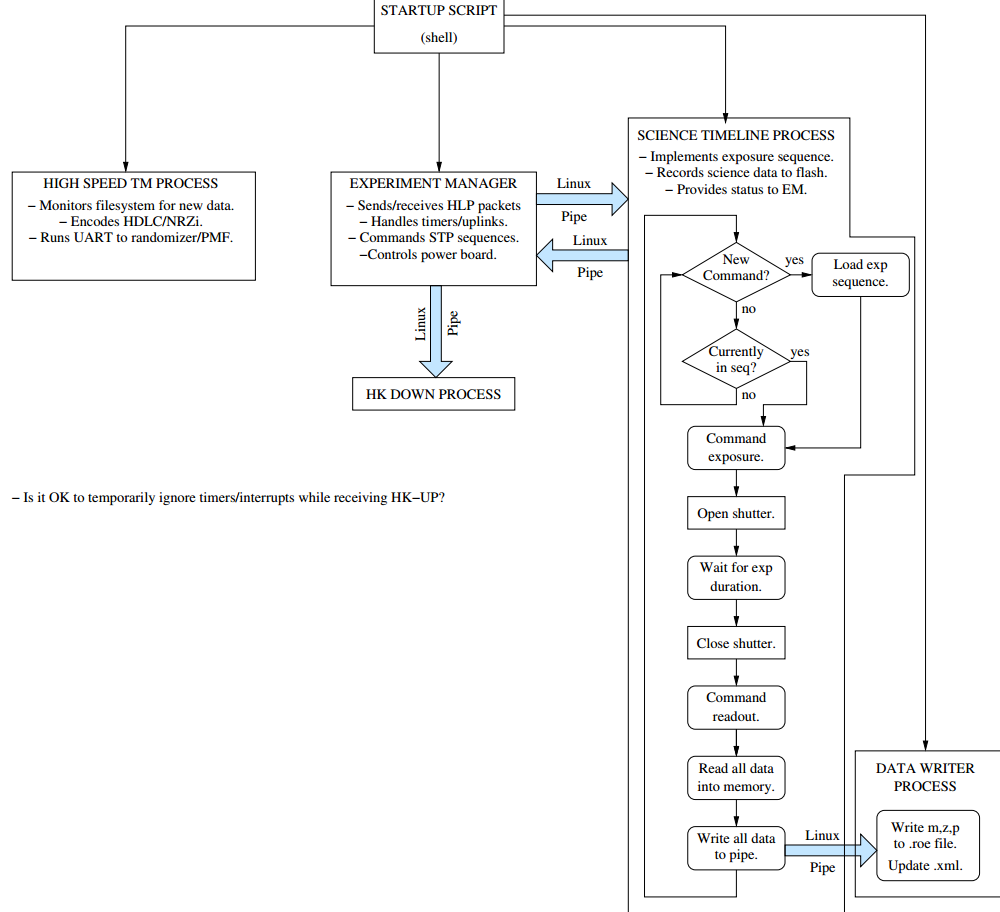
\includegraphics{software.png}}
\end{minipage}
\end{tabular}
}


%%%%%%%%%%%%%%%%%%%%%%%%%%%%%%%%%%%%
%          First Column            %
%%%%%%%%%%%%%%%%%%%%%%%%%%%%%%%%%%%%

\headerbox{Hardware Specifications}{name=Experimental Design,column=1,span=3}{
\begin{tabular}{ll}
  \begin{minipage}{.4\columnwidth}
    \resizebox{1\columnwidth}{!}{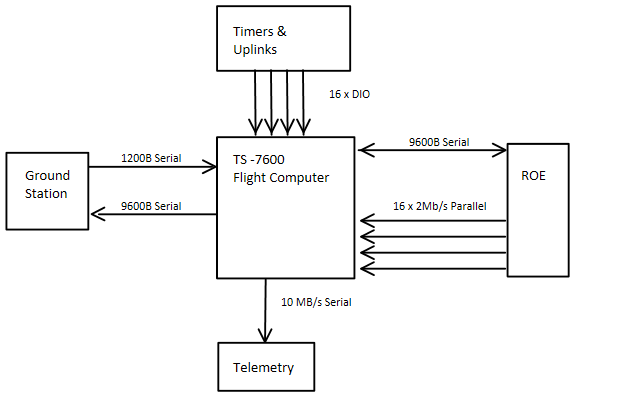
\includegraphics{functionalDiagram}}
    \footnotesize{Flight Computer Functional Diagram}  
 \end{minipage}&
 \begin{minipage}{.55\columnwidth}

Success of the mission requires that many different components of the payload communicate effectively. The experiment must start at the right time, collect exposures of the sun and  send them back to earth. Coordination with the rocket is achieved through timing signals provided by NASA. During normal operation, the timers control the experiment, informing the computer when to take each exposure. Also present on the same interface are uplinks, that correspond to signals that can be sent from the ground to provide control. The camera interface is provided by two connections to the read-out electronics (ROE). The first connection is a serial connection which is used to control the cameras, while the second is a 16 bit parallel connection that sends images  back to the computer. Once these images are saved to disk, they are transmitted back to earth via a 10 MB/s telemetry connection. To provide additional control during flight, a housekeeping link is provided between a ground station computer and the flight computer. This link provides up-to-date information about the state of the flight computer and the various subsytems on the payload.


\end{minipage}
\end{tabular}
}

\headerbox{Housekeeping Software}{name=mounts,column=1,span=2, below=Experimental Design,above=concept}{
\begin{tabular}{ll}
  \begin{minipage}{0.55\columnwidth}
     Communication between computers on the ground and the flight computer is accomplished through a two-way housekeeping link. Both computers communicate using the housekeeping-link protocol (HLP), which outlines a packet structure that can be understood by both machines. Housekeeping packets contain commands that allow operators on the ground to observe real-time mission data, change the sequence of pictures, and control the flight computer using a command line interface.

  \end{minipage}&
  \begin{minipage}{0.35\columnwidth}
      \resizebox{\columnwidth}{!}{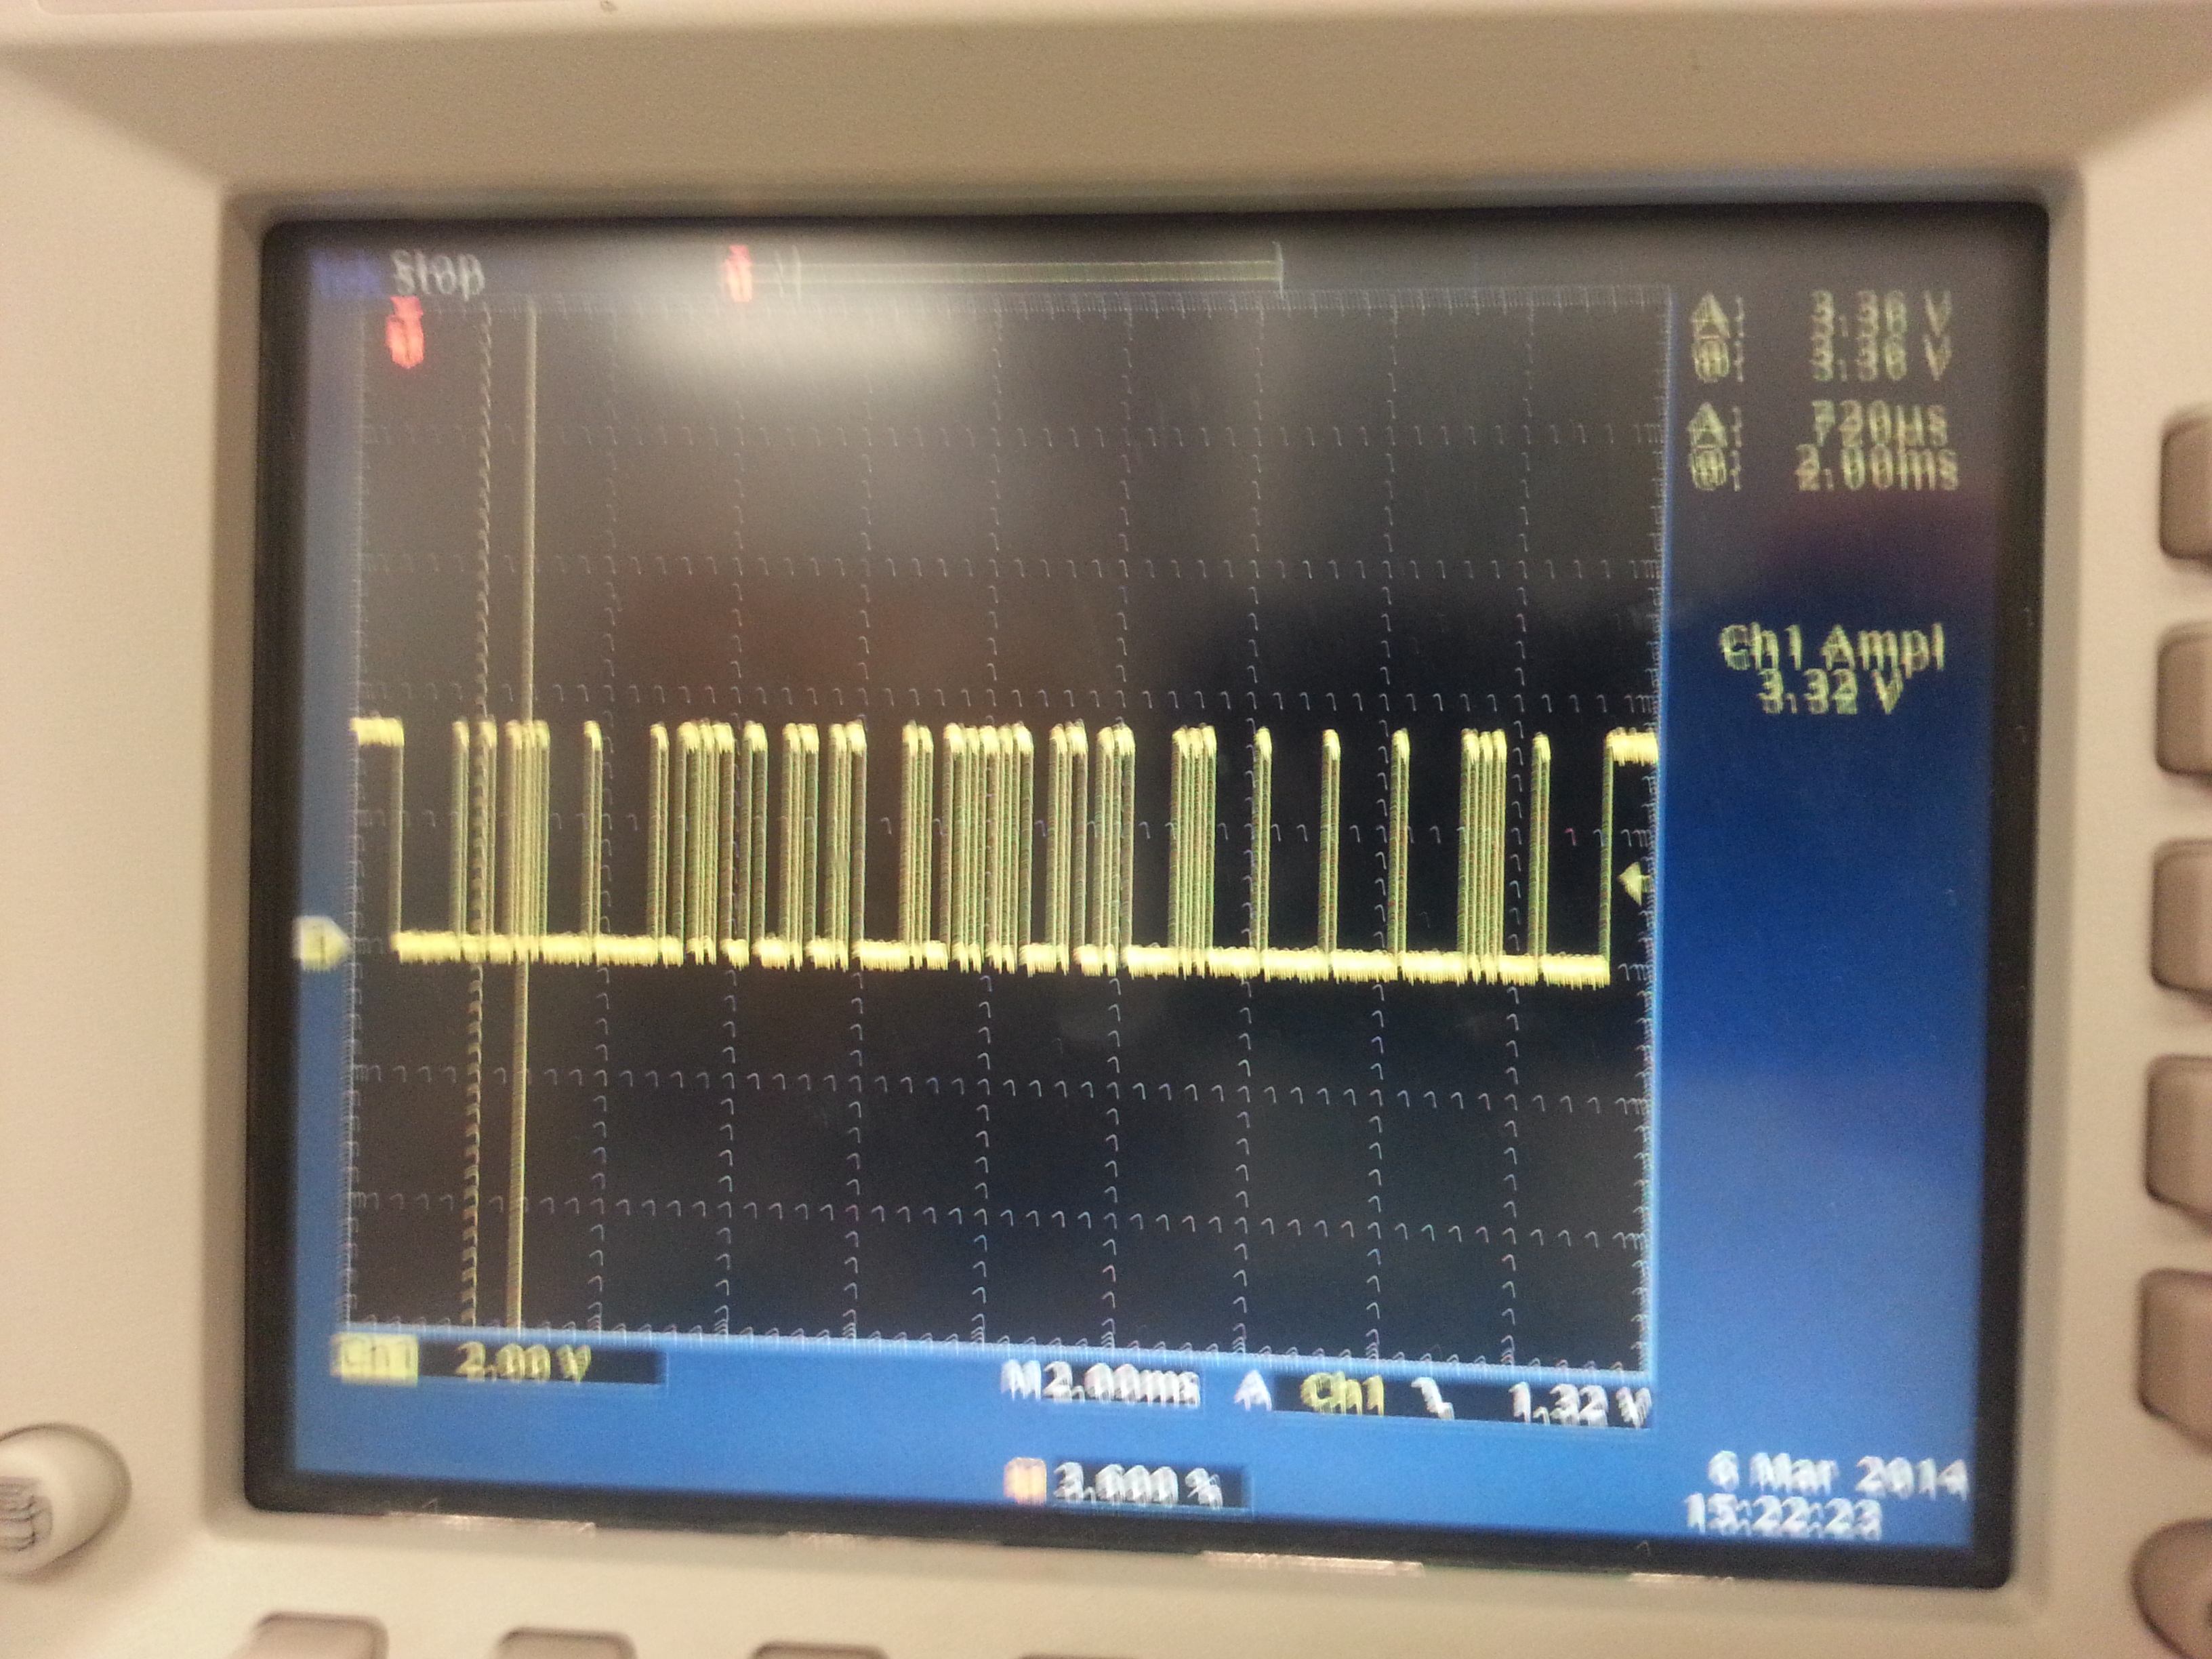
\includegraphics{hkOscilloscope.jpg}}
      \footnotesize{HK packet on Oscilloscope}  
\end{minipage}  
\end{tabular}

}

%%%%%%%%%%%%%%%%%%%%%%%%%%%%%%%%%%%%
%          Second Column           %
%%%%%%%%%%%%%%%%%%%%%%%%%%%%%%%%%%%%

\headerbox{Complications}{name=HCL,column=2,span=1,below=mounts}{

Specifications provided for the TS-7600 vastly overestimated the capabilities of the throughput through the onboard FPGA. Through experimentation, it was discovered that the planned interfaces for both the high-speed TM and 16-bit parallel image data were unable to complete transfers within the mission requirements. A SyncLink USB serial adapter was purchased that addressed the high-speed TM. Image data acquisition has yet to be solved.

\begin{center}
\footnotesize{SyncLink USB Adapter}
\resizebox{.20\columnwidth}{!}{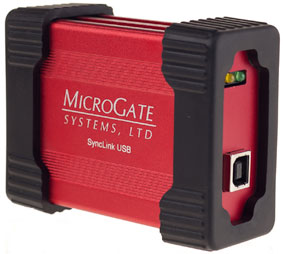
\includegraphics{usb.jpg}}

\end{center}

}




%%%%%%%%%%%%%%%%%%%%%%%%%%%%%%%%%%%%
%          Third Column            %
%%%%%%%%%%%%%%%%%%%%%%%%%%%%%%%%%%%%

\headerbox{Development Schedule}{name=GSE,column=3,below=Experimental Design}{
\begin{center}
   \resizebox{0.8\columnwidth}{!}{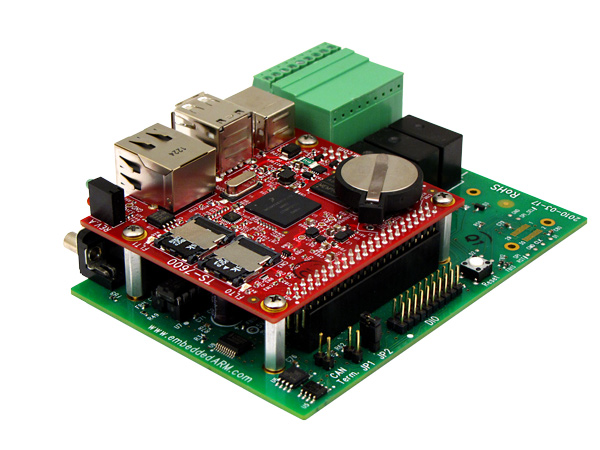
\includegraphics{ts7600.jpg}}\\
   \footnotesize{TS-7600 Flight Computer}
\end{center}
Much of the code has yet to be developed. Only the experiment manager is in an advanced state of development. Features missing from the program are any communications with the ROE, timers and uplinks. Programs need to be developed to execute the science timeline process and the high-speed TM process.

}

\headerbox{Acknowledgment}{name=ack,column=3,below=GSE}{ \footnotesize
This work is supported by MSU USP and MSGS.
\normalsize}


\headerbox{References}{name=refs,column=3,below=ack,above=bottom}{\footnotesize
\begin{minipage}{\columnwidth}
[0]Kankelborg, \textit{Simultaneous Imaging and Spectroscopy of The Solar Atmosphere}
 
\end{minipage}
\normalsize}


\end{poster}

\end{document}